\begin{definition}  \textbf{Rect\'angulo.} Al conjunto \( B  \subseteq  \mathbb{R}^2 \) dado por
	\[
	B = [a, b] \times [c, d] = \{(x, y) \in \mathbb{R}^2 \mid a \leq x \leq b, \; c \leq y \leq d\}
	\]
	se lo llama rect\'angulo.   
\end{definition}	

\begin{definition} \textbf{Partici\'on regular.} 	Sea \( B  \subseteq  \mathbb{R}^2 \) un rect\'angulo.  Una partición regular de $B$ es un conjunto de pequeños rectángulos disjuntos (salvo tal vez por sus bordes)  de igual \'area que  generan una subdivisi\'on de $B$.  Es decir, si $B = [a, b] \times [c, d]$,  esto se logra dividiendo:
	
	\begin{itemize}
		\item el intervalo \( [a, b] \) en \( n \) subintervalos \( [x_i, x_{i+1}] \) con $0 \leq  i \leq n-1$, cada uno de ancho \( \Delta x \),
		\item el intervalo \( [c, d] \) en \( m \) subintervalos \( [y_j, y_{j+1}] \) con $0 \leq  j \leq m-1$, cada uno de ancho \( \Delta y \).
	\end{itemize}
y tomando los subrect\'angulos $B_{ij}$ tales que
	\[
	B_{ij} = [x_i, x_{i+1}] \times [y_j, y_{j+1}], 
	\]  El \'area de $ B_{ij}$ la notaremos por $\Delta B_{ij}$ 
\end{definition}


\begin{definition}
Dada una funci\'on $f:B\to\R$, donde $B$ es un rect\'angulo en $\Rn{2}$, se define la suma de Reimann de $f$ sobre $B$ a 
\[
    S_{n,m}=\sum_{i=0}^{n-1}\sum_{j=0}^{m-1} f(c_{ij})\Delta B_{ij},
\]  
donde $\{ B_{ij}\}_{( 1 \leq i \leq n, 1 \leq j \leq m )}$ es una partici\'on regular de $B$ y  $c_{ij}\in B_{ij} \: \forall \: 1 \leq i \leq n, 1 \leq j \leq m$. 
\end{definition}

\begin{definition} 
    Sea $f:B=[a,b]\times[c,d]\to\R$ una funci\'on. Diremos que $f$ es integrable sobre $B$ si  el l\'imite $\lim_{(n,m)\to (\infty,\infty)}S_{n,m}$  existe y es finito, en tal caso el valor de dicho  l\'imite  se llama \textbf{integral doble} de $f$ sobre $B$ y se nota 
    \[
          \iint_B f\:dA  \mbox{ o } \iint_B f(x,y)\:dxdy.
    \]
\end{definition}

\begin{obs}
Para que exista el límite,  es suficiente que $f$ sea acotada sobre el rectángulo $B$, y el conjunto de puntos de (posibles) discontínuidades  sea la unión finita de gráficas
de funciones continuas. Es decir, $f$ contínua, excepto, tal vez, sobre curvas.
\end{obs}


Para extender esta noci\'on de integral a  conjuntos acotados m\'as generales que no sean  rect\'angulos, definimos lo siguiente. 

\begin{definition}\label{def:int_D}
Sean $D  \subseteq  \mathbb{R}^{2}$,  $f:D \to\R$ contínua y $R=[a,b]\times[c,d]$ tal que $D  \subseteq  R$.  Se define la funci\'on $f^*$ tal que 
\[
    f^*(x,y)=
    \begin{dcases*}
        f(x,y) & si $(x,y)\in D$ \\[.2cm]
        0        & si $(x,y)\in R \setminus D.$
    \end{dcases*}
\]

Dada su definici\'on, $f^*$ no tiene porque ser continua sobre todo $R$ pero de tener discontinuidades  las mismas estar\'an sobre  $\partial D$. Luego, si $\partial D$ est\'a formada por una curva continua entonces $f^*$ es integrable y  se define la integral de $f$ sobre $D$ por
\[
    \iint_D f\:dA=\iint_B f^*\:dA.  
\]
\end{definition}
La explicación se puede observar mejor en la siguiente figura:


 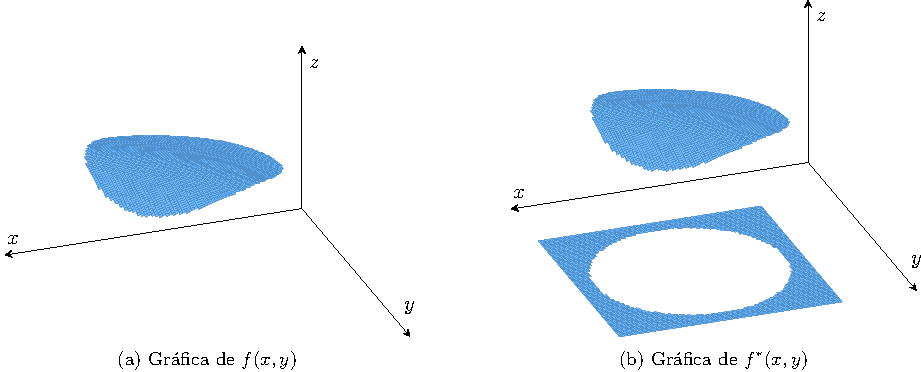
\includegraphics{standalone_fig_integral.pdf}

%\begin{figure}[H]
 %   \centering
 % === Subfigura (a) ===
 %   \begin{subfigure}[b]{0.45\textwidth}
 %   \centering
  %  \begin{tikzpicture}
  %  \begin{axis}[
    %    view={160}{40},
     %   xmin=0, xmax=2,
   %     ymin=0, ymax=2,
    %    zmin=0, zmax=3,
     %   axis lines=center,
     %   ticks=none,
     %   xlabel={$x$}, ylabel={$y$}, zlabel={$z$},
     %   domain=0:2, y domain=0:2,
     %   samples=30, z buffer=sort
  %  ]
        % Región R (rectángulo base)
     %   \addplot3[
    % surf,
  %  shader=faceted,
  %  draw=black, % dibuja las líneas de la malla
   % fill=gray, fill opacity=0.2,
  %  domain=0.5:2, y domain=0.5:2,
  %  samples=20
%] {0};

    %    % Superficie sobre región R (solo en R)
     %   \addplot3[
      %      surf, opacity=0.7, colormap={mycolor}{rgb255=(100,180,255) rgb255=(100,180,255)},
        %    domain=0.5:2, y domain=0.5:2,
      %  ] {sin(x*y*50)+2};
   % \end{axis}
   % \end{tikzpicture}
    % \caption{Gráfica de \( f(x,y) \) sobre  \( R \)}
    % \end{subfigure}
    % \hfill
    % === Subfigura (b) ===
    % \begin{subfigure}[b]{0.45\textwidth}
   % \centering
   % \begin{tikzpicture}
   % \begin{axis}[
     %   view={160}{40},
     %   xmin=0, xmax=2,
     %   ymin=0, ymax=2,
     %   zmin=0, zmax=3,
     %   axis lines=center,
      %  ticks=none,
      %  xlabel={$x$}, ylabel={$y$}, zlabel={$z$},
       %  domain=0:2, y domain=0:2,
      %  samples=60, z buffer=sort
   % ]

     %   % Superficie f(x,y) sobre toda R, con 0 fuera de D
     %   \addplot3[
       %     surf, opacity=0.8,
      %      domain=0.5:1.5, y domain=0.5:1.5,
       %     colormap={mycolor}{rgb255=(100,180,255) rgb255=(100,180,255)},
        %     restrict z to domain=2.1:10, % recorta para evitar planicies
   % unbounded coords=jump,
    %    ]
      %  { ( (x-1)^2 + (y-1)^2 < 0.2 ) * sin(x*y*50)+2 };

         % Región R en gris claro
     % \addplot3[
   % surf,
  %  shader=faceted,
   % draw=black, % dibuja las líneas de la malla
   % fill=gray, fill opacity=0.2,
   % domain=0.5:2, y domain=0.5:2,
  %  samples=20
%] {0};
        
       % \addplot3[
        %    surf, opacity=0.8,
         %   domain=0.5:2, y domain=0.5:2,
        %    colormap={mycolor}{rgb255=(100,180,255) rgb255=(100,180,255)},
      %       restrict z to domain=-0.1:0.1, % recorta para evitar planicies
  %  unbounded coords=jump,
      %  ]
      %  { ( (x-1)^2 + (y-1)^2 < 0.2 ) + 0 };

  %  \end{axis}
   % \end{tikzpicture}
  %  \caption{Gráfica de \( f^*(x,y) \) sobre \( R \)}
  %  \end{subfigure}
%\end{figure}

























\begin{obs} 
La  \autoref{def:int_D}  es independiente  de la selecci\'on de $B$.
\end{obs}

\begin{propertie}
    Sean $f,\;g$ dos funciones integrables en una regi\'on $D\subset\Rn{2}$, entonces:
    \begin{enumerate}
        \item[i.] $\alpha f+\beta g$ es integrable en $D$, $\forall\;\alpha,\;\beta\in\R$ y, adem\'as,
        \[
            \iint_D \left(\alpha f+\beta g\right)dA=\alpha\iint_D f\:dA+\beta\iint_D g\:dA.
        \]
        \item[ii.] El producto $fg$ es integrable en $D$.
        \item[iii.] Si $g(x,y) \neq 0\;\forall(x,y)\in D$ entonces el cociente $f/g$ es integrable en $D$.
        \item[iv.] Si $f(x,y)\geq 0 \;\forall(x,y)\in D$ entonces  $\iint_D f\:dA\geq0$.
        \item[v.]Si $f(x,y)\leq g(x,y)  \;\forall(x,y)\in D$ entonces $\iint_D f\:dA\leq\iint_D g\:dA.$
        \item[vi.]Si $|f|$ es integrable en $D$ entonces 
        \[
            \left|\iint_D f\:dA\right|\leq\iint_D|f|\:dA.  
        \]    
        \item[vii.] Si $D=D_1\cup D_2$ donde $\;D_1\cap D_2$ es un conjunto de medida nula  entonces   $f$ es integrable sobre $D_1$ y sobre $D_2$ y, adem\'as,  
        \[
            \iint_D f\:dA=\iint_{D_1} f\:dA+\iint_{D_2}f\:dA.    
        \]
    \end{enumerate}
\end{propertie}

%-----------------------------------------------------------
\begin{definition}\label{conj_elem}  Un conjunto  $D\subseteq\Rn{2}$ se llama elemental si  puede ser descripto de alguna de las siguientes maneras. 
   
    \begin{enumerate}
    \item[i.]  Existen funciones $\phi_1,\;\phi_2:[a,b]\to\R$  continuas  tales que $ \phi_1(x) < \phi_2(x) \: \forall x \in (a,b) $  y:
    \[
     D = \{ (x,y) \in \mathbb{R}^{2}: \:   x\in[a,b] \: \land \: \phi_1(x)\leq y\leq\phi_2(x) ;\forall\;x\in[a,b] \}  
    \]   En tal  el conjunto $D$ se llama  \textit{elemental de tipo 1.} 
   
    \item[ii.]  Existen funciones $\psi_1,\;\psi_2:[c,d]\to\R$  continuas tales que $ \psi_1(y) < \psi_2(y) \: \forall y \in (c,d)$ y 
    \[
     D = \{ (x,y) \in \mathbb{R}^{2}:   y\in[c,d] \: \land \:  \psi_1(y)\leq x\leq\psi_2(y) ;\forall\;y\in[c,d] \}  
    \]
     En tal  el conjunto $D$  se llama  \textit{elemental de tipo 2.} 
    
    \item[iii.] $D$ se llama conjunto elemental de \textit{tipo 3} si es \textit{tipo 1} y \textit{tipo 2} a la vez.
    
    \input{figs/conj-elementales.tex}
    
    \end{enumerate}
\end{definition}

\begin{example}
    Para poder clasificar a una regi\'on como tipo 3 es necesario poder encontrar simult\'aneamente funciones $\phi_1$, $\phi_2$, $\psi_1$ y $\psi_2$ tales que
    \[
    \begin{dcases}
        \phi_1(x)\leq y\leq\phi_2(x) & x\in[a,b]\\[.2cm]
        \psi_1(y)\leq x\leq\psi_2(y) & y\in[c,d].
    \end{dcases}
    \]
    Un ejemplo simple de tal regi\'on es un c\'irculo, donde la ecuaci\'on de esta regi\'on es $$D=\{(x,y)\in\Rn{2}:(x-x_0)^2+(y-y_0)^2\leq r\}.$$  

    \input{figs/ex_tipo3.tex}

    Para esta regi\'on se pueden encontrar las funciones
    \[
        \phi_1(x)=-\sqrt{r-(x-x_0)^2}+y_0,\quad x\in[x_0-r,x_0+r],
    \]
    y
    \[
        \phi_2(x)=\sqrt{r-(x-x_0)^2}+y_0,\quad x\in[x_0-r,x_0+r].
    \]
    A su vez, se pueden hallar las funciones
    \[
        \psi_1(y)=-\sqrt{r-(y-y_0)^2}+x_0,\quad y\in[y_0-r,y_0+r],
    \]
    y
    \[
        \psi_2(y)=\sqrt{r-(y-y_0)^2}+x_0,\quad y\in[y_0-r,y_0+r].
    \]
    Por tanto, $D$ es una regi\'on de tipo 3.
\end{example}


\begin{theorem}  \label{col:fubini} \textbf{Teorema de Fubini} en $\mathbb{R}^{2}.$  Sea $f:D\to\R$ continua sobre  $D\subseteq\Rn{2}$  un conjunto elemental   (\ref{conj_elem}) 
   
\begin{enumerate} 
        \item  Si $D$ es de tipo 1   entonces la integral doble de $f$ sobre $D$ se puede calcular
        \[
            \iint_D f=\int_a^b\left(\int_{\phi_1(x)}^{\phi_2(x)}f(x,y)\:dy\right)dx.  
        \]
       
        \item   Si $D$ es de tipo 2   entonces la integral doble de $f$ sobre $D$ se puede calcular
        \[
            \iint_D f=\int_a^b\left(\int_{\psi_1(y)}^{\psi_2(y)}f(x,y)\:dx\right)dy.  
        \]
       
        \item Si $D$ es de tipo 3   entonces la integral doble de $f$ sobre $D$ se puede calcular  
         \[
            \iint_D f=\int_a^b\left(\int_{y=\phi_1(x)}^{y=\phi_2(x)}f(x,y)\:dy\right)dx=\int_a^b\left(\int_{x=\psi_1(y)}^{x=\psi_2(y)}f(x,y)\:dx\right)dy. 
        \]
    \end{enumerate}
\end{theorem}


\begin{obs} La \'unica manera de demostrar que un conjunto es elemental es dando su descripci\'on  impl\'icita.
\end{obs}


\begin{example}
     Sean $f(x,y)=x^2y$ y  $D$ es la regi\'on del plano encerrada por $y=x^3$, $y=x^2$  con $x\in[0,1]$,  calcular,  $$\iint_D f \:dA.$$  

    \begin{center}
    \begin{tikzpicture}
        \begin{axis}[
            axis lines = middle,
            xmin = 0, xmax = 1.5,
            ymin = 0, ymax = 1.5,
            xlabel = {$x$},
            ylabel = {$y$},
            domain = 0:1.25,
            samples = 100,
            xtick={0.5,1},
            ytick={0.5,1},
            clip=false,
            ]
        
            % Define the curves
            \addplot[name path=A, blue, thick, domain=0:1.22] {x^2} node[pos=0.75, right] {$y=x^2$};
            \addplot[name path=B, red, thick, domain=0:1.15] {x^3} node[pos=0.3, below right] {$y=x^3$};
        
            % Fill the area between the curves
            \addplot[orange!50, fill opacity=0.5] fill between[of=A and B, soft clip={domain=0:1}];
        
            % Label the enclosed area as D
            \node at (axis cs:0.6,0.29) {$D$};
        
        \end{axis}
    \end{tikzpicture}
    \end{center}

 $D$ puede ser descripto de la siguiente manera
    \[
        D=\{(x,y)\in\Rn{2}:0\leq x\leq1;\;x^3\leq y\leq x^2\},  
    \]
 luego $D$ es elemetal de tipo 1 y  por el \autoref{col:fubini}
    \begin{gather*}
        \iint_D x^2y\:dA=\int_0^1\left(\int_{x^3}^{x^2}\:dy\right)dx=\int_0^1\left(x^2\frac{1}{2}y^2\Big\lvert_{x^3}^{x^2}\right)dx\\
        =\int_0^1\frac{1}{2}x^2\left((x^2)^2-(x^3)^2\right)=\int_0^1\frac{1}{2}x^6-\frac{1}{2}x^8\;dx\\=\frac{1}{14}x^7-\frac{1}{18}x^9\Big\lvert_0^1=\frac{1}{14}-\frac{1}{18}=\frac{1}{63}.
    \end{gather*}
\end{example}

\begin{tarea}Calcular  $$ \int_{0}^{1}\int_{y}^{1} e^{x^{2}} \:\: dx\:dy $$
\end{tarea}



\begin{definition}  Sea $D\subset\Rn{2}$,  se define el \'area de $D$,  y se nota $\text{A}(D)$,  a  
    \[
        \text{A}(D)=\iint_D1\:dA.
    \]
\end{definition}



\begin{theorem}
    \textbf{Teorema del valor medio para integrales dobles.}   Sea $f:D\subseteq\Rn{2}\to\R$ continual.  Entonces existe $(x_0,y_0)$ en $D$ tal que
    \[
        \int_D f(x,y)\:dA=f(x_0,y_0)\text{A}(D).
    \]
\end{theorem}

\begin{definition}
    Sea $\mathbf{F}:A\subseteq\Rn{n}\to\Rn{n}$ un campo $\mathcal{C}^1(A)$ y sea $\boldsymbol{D}_\mathbf{F}$ (\autoref{def:mat_dif}) su matriz diferencial.  Se define el \emph{jacobiano}, o \emph{determinante jacobiano}, y se lo nota $J_\mathbf{F}$ a 
    \[
        J_\mathbf{F}=\text{det}(\boldsymbol{D}_\mathbf{F}).
    \]
\end{definition}


\begin{example}  Calcular $J_\mathbf{F}$ siendo  \( \mathbf{F}(r, \theta) = (r\cos\theta, r\sin\theta) \).

 Primero, calculamos su la matriz diferencial.
       \[
       \boldsymbol{D}_{\mathbf{F}}(r, \theta) 
       =
       \begin{bmatrix}
       \cos\theta & -r\sin\theta \\
       \sin\theta & r\cos\theta
       \end{bmatrix}
       \]
       Entonces, el jacobiano es
       \[
       J_{\mathbf{F}}(r, \theta) = \det(\boldsymbol{D}_{\mathbf{F}})(r, \theta) = 
      r(\cos^2\theta + \sin^2\theta) = r.
       \]
   \end{example}
   
   \begin{example}  Calcular $J_\mathbf{F}$   siendo   \( \mathbf{F}(r, \theta, z) = (r\cos\theta, r\sin\theta, z) \).
        
  Primero, calculamos su la matriz diferencial.
   \[
    \boldsymbol{D}_{\mathbf{F}} (r, \theta,  z)=
    \begin{bmatrix}
   \cos\theta & -r\sin\theta & 0 \\
   \sin\theta & r\cos\theta & 0 \\
   0 & 0 & 1
   \end{bmatrix}
   \]   
    Entonces, el jacobiano es 
   
   \[
   J_\mathbf{F} (r, \theta, z) = \det(D_F)(r, \theta, z)  = 
   \begin{vmatrix}
   \cos\theta & -r\sin\theta & 0 \\
   \sin\theta & r\cos\theta & 0 \\
   0 & 0 & 1
   \end{vmatrix}
   = r
   \]
   \end{example}
   
   \begin{example}  Calcular $J_\mathbf{F}$   siendo  \( \mathbf{F}(\rho, \theta, \phi)  = (\rho\sin\phi\cos\theta, \rho\sin\phi\sin\theta, \rho\cos\phi) \). 
   
   
    Primero, calculamos su la matriz diferencial.
   
    \[
    \boldsymbol{D}_{\mathbf{F}}(\rho, \theta, \phi) 
    =
    \begin{bmatrix}
    \sin\phi \cos\theta & -\rho \sin\phi \sin\theta & \rho \cos\phi \cos\theta \\
    \sin\phi \sin\theta & \rho \sin\phi \cos\theta & \rho \cos\phi \sin\theta \\
    \cos\phi & 0 & -\rho \sin\phi
    \end{bmatrix}
    \]
     Entonces, el jacobiano es 
    
    \[
    J_\mathbf{F}(\rho, \theta, \phi)  = \det(\boldsymbol{D}_{\mathbf{F}})(\rho, \theta, \phi)  = \begin{vmatrix}
        \sin\phi \cos\theta & -\rho \sin\phi \sin\theta & \rho \cos\phi \cos\theta \\
        \sin\phi \sin\theta & \rho \sin\phi \cos\theta & \rho \cos\phi \sin\theta \\
        \cos\phi & 0 & -\rho \sin\phi
        \end{vmatrix}=\rho^2 \sin\phi
    \]
    
    
    \end{example}

\begin{theorem} % lo escribi como lo tenia en mis apuntes
    \textbf{Teorema del cambio de variables para integrales dobles.}   Sean $D \subseteq\Rn{2}$ un conjunto acotado y  $f:D \to\R$ un campo integrable sobre $D$   y sea $\mathbf{T}:D^*\subseteq\Rn{2}\to D$ continua en $D^*$,  de clase $\mathcal{C}^1(\interior{(D^*)})$,  inyectiva en $\interior{(D^*)}$ y tal que $\mathbf{T}(D^*)=D$. Entonces
    \[
        \iint_D f\:dA=\iint_{D^*}(f\circ\mathbf{T})|J_\mathbf{T}|\:dA,
    \]
    donde $|J_\mathbf{T}|$ es el m\'odulo del jacobiano de $\mathbf{T}$.
\end{theorem}


 \begin{example} Hallar el \'area de la regi\'on $$ D=\{(x,y)\in\Rn{2}: \: 1 \leq x^{2}+ y^{2}  \leq4 \}.$$ 
 \end{example} 
